	\section{Modello di sviluppo}
Come \glo{team} di sviluppo dobbiamo poter garantire in ogni momento la qualità del prodotto \glo{software} e la sua conformità rispetto ai \glo{requisiti}. Ciò è permesso dal modello \glo{agile}, che favorisce un ciclo evolutivo più flessibile e il dialogo con gli \glo{stakeholder}, adattandosi più facilmente alle esigenze. Per tali motivi abbiamo deciso di adottare questo tipo di modello, riducendo i rischi e producendo nuovo valore ad ogni \glo{sprint}.
\newline

%info
%https://medium.com/geekandjob-blog/scrum-cos%C3%A8-e-come-funziona-metodologia-agile-7c8988feec01
\subsection{Modello Agile}
Il modello di sviluppo \glo{agile} permette di progredire tramite cicli iterativi, detti \glo{sprint}.
É un modello altamente dinamico concepito per evitare un'eccessiva rigidità, valorizzando le risorse disponibili. \newline
Il manifesto \glo{agile} contiene quattro principi fondanti:

\begin{enumerate}
    \item \textbf{Gli individui e le interazioni più che i processi e gli strumenti}: le persone che fanno parte del progetto producono valore e sono una grande risorsa disponibile;
    \item \textbf{Il \ignore{software} funzionante più che la documentazione esaustiva}: la documentazione va snellita e resa più flessibile senza però perderne in qualità, allocando più risorse al \glo{software};
    \item \textbf{La collaborazione con il cliente più che la negoziazione dei contratti}: un contratto inflessibile può essere una potenziale perdita di valore per per tutte le parti coinvolte. Va quindi incentivata l'interazione con gli \glo{stakeholder} durante lo sviluppo del progetto;
    \item \textbf{Rispondere al cambiamento più che seguire un piano}: i cambiamenti sono probabili durante lo sviluppo di grandi progetti, per questo, pianificare tutto fin dall'inizio potrebbe essere uno spreco di risorse.
\end{enumerate}
L'idea di base per implementare tali principi è l'utilizzo del \textbf{\glo{Product Backlog}}, che cresce man mano che il prodotto viene costruito. \newline
Il lavoro viene quindi suddiviso in piccole funzionalità chiamate \textbf{\glo{User Story}}, le quali poi vengono selezionate per essere portate a termine negli \textbf{\glo{sprint}}, venendo, di fatto, sviluppate indipendentemente in una sequenza continua dall'analisi all'integrazione. \newline

Gli obiettivi strategici quindi sono:
\begin{itemize}
    \item poter dimostrare costantemente e in ogni momento ciò che è stato fatto al cliente;
    \item verificare l'avanzamento tramite il progresso reale dello sviluppo;
    \item soddisfare e motivare gli sviluppatori con risultati immediati;
    \item assicurare e dimostrare una buona \glo{verifica} e integrazione dell'intero prodotto \glo{software}.
\end{itemize}
I \textbf{vantaggi} principali di questo modello sono, come riportato sopra, la facilità di adattamento in base alle esigenze da parte del \glo{team}, 
una grande dinamicità nel gestire i cambiamenti, progredendo con piccoli incrementi di valore aggiunto,
e la grande attenzione posta alla comunicazione sia interna che esterna con tutti gli \glo{stakeholder} facendo sì che le richieste di \proponente{} vengano soddisfatte a pieno.

\begin{figure}[H]
    \centering
    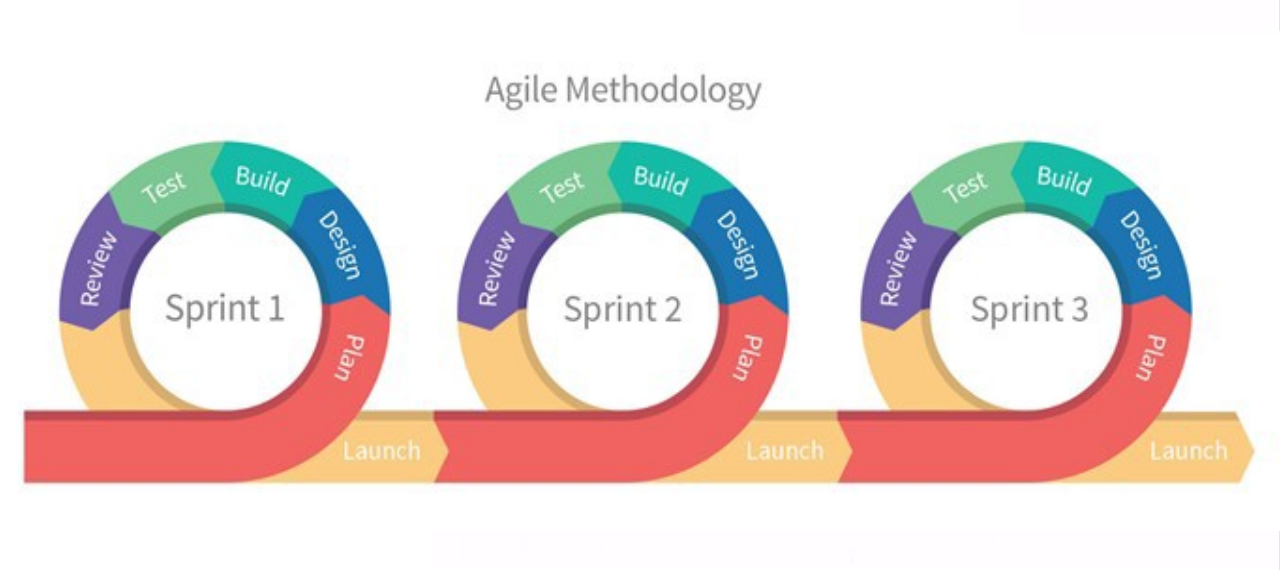
\includegraphics[scale = 0.25]{components/img/agile.png}
    \caption{Rappresentazione del modello agile}
    \label{fig:Rappresentazione del modello agile}
\end{figure}


\subsection{Modalità realizzativa}
Nel contesto del progetto in questione, il modello di sviluppo \glo{agile} sarà adottato dai membri
del \glo{team} secondo i seguenti punti cardine:
\begin{itemize}
    \item \textbf{\ignore{Sprint}}: Il periodo di sviluppo \glo{software} del prodotto sarà caratterizzato dal susseguirsi di \glo{sprint} di 2 settimane. Ogni \glo{sprint} dovrà essere inizialmente pianificato sulla base delle attività con priorità maggiore, e dovrà concludersi obbligatoriamente nel lasso di tempo prestabilito. Ogni \glo{sprint} caratterizzerà un incremento, anche parziale, del valore aggiunto del prodotto;
    \item \textbf{Riunioni settimanali}: I membri del \glo{team} si impegnano ad effettuare un incontro settimanale, nella quale ci si aggiorna sullo stato di avanzamento dei lavori o su eventuali problematiche incontrate durante lo sviluppo;
    \item \textbf{Coinvolgimento degli \ignore{stakeholder}}: Per l'attuazione del modello di sviluppo \glo{agile} è fondamentale avere un feedback costante da parte degli \glo{stakeholder}. Per questo motivo, ogni scelta implementativa e realizzativa presa dal \glo{team}, dovrà essere confermata da questi ultimi;
    \item \textbf{Aggiornamento giornaliero}: Ogni membro del gruppo \gruppo{} si impegna a fornire ai propri collaboratori aggiornamenti quotidiani sullo stato di progresso della parte assegnatagli, così da diminuire la probabilità di rischi correlati alla poca trasparenza;
    \item \textbf{Discussione feedback}: Durante l'ultimo giorno di \glo{sprint}, il \glo{team} dovrà quantificare e valutare obiettivamente il lavoro svolto in quel periodo di tempo, oltre a dover proporre migliorie o altre caratteristiche da implementare.
\end{itemize}